%pme2360
\section{Exercício}

% \begin{figure}[h]
% \begin{center}
% 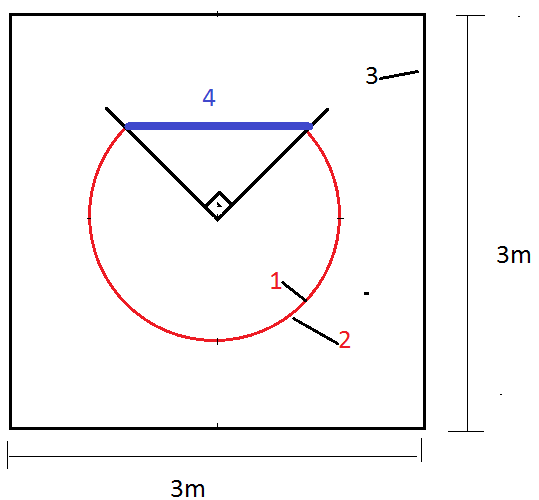
\includegraphics[scale=0.28]{./fig/1.png}
% \caption{\label{fig:1}1} 
% \end{center}
% \end{figure}

\myfig[scale=.28]{figPME2360-20111130-01}{}

\[\dot{m}_{oleo}=2Kg/s\]
\[T_{h,i} = 120ºC\]
\[T_{h,o} = 40ºC\]
\[c_{p,oleo} = 2118.0 J/kg\]

\[U = 3000 W/m^{2}K\]
\[T_{c,i} = 15ºC\]
\[T_{c,o}= 45ºC\]
\[c_{p,agua} = 4178 J/kg\]

\subsection{a}
\textit{vazão mássica de água}
\[\dot{m}_{oleo} \times c_{p,oleo} (T_{h,i}-T_{h,o}) = \dot{m} \times c_{p,agua}(T_{c,o}-T_{c,i})\]
\[2 \times 2118 \times (120-40) = \dot{m} * 4178 * ( 45-15 ) = \dot{q}=33880J/kg\]
\[\dot{m}_{agua}=2.70 \ kg/s\]

\subsection{b}
Trocador de casco-tubo

1 passe na carcaça

6 passes nos tubos

% \begin{figure}[h]
% \begin{center}
% 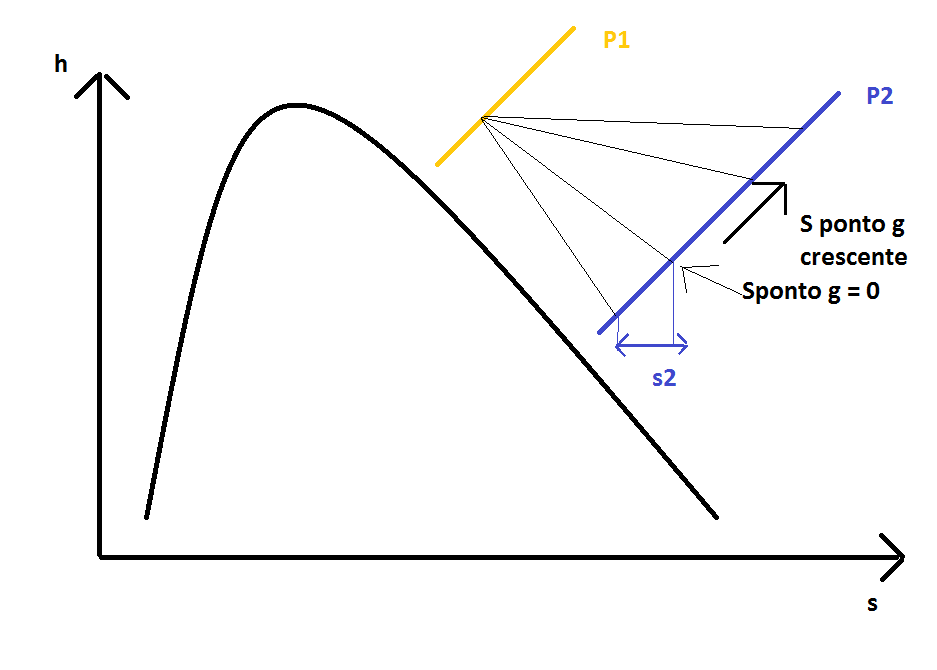
\includegraphics[scale=0.28]{./fig/2.png}
% \caption{\label{fig:2}Trocador em contra-corrente} 
% \end{center}
% \end{figure}

\myfig[scale=.28]{figPME2360-20111130-02}{}

\paragraph{Método MLDT}
Método Logarítmo para trocador de calor em corrente contrária

\[\Delta T_{lm,cc}=\frac{\Delta T_{1}-\Delta T_{2}}{\ln(\Delta T_{1}/\Delta T_{2})}\]
Em que lm é a média logarítmica e o cc é a corrente contrária

\[\Delta T_{1} = T_{h,i} - T_{c,o} = 120 - 45 = 75\]
\[\Delta T_{2} = T_{h,o} - T_{c,i} = 40 - 15 = 25\]

\[\Delta T_{lm,cc} = \frac{75-25}{\ln(75/25)}=45.5ºC\]

\[q = UA \Delta T_{lm,cc} F\]

Pela figura 11.10, (pag 459, 5a ed.)

\myfig[scale=.28]{figPME2360-20111130-03}{}

\[R = \frac{T_{e}-T_{s}}{t_{s}-t_{e}} = \frac{120-45}{45-15}=2.66\]
\[P = \frac{t_{s}-t_{e}}{T_{e}-t_{e}} = \frac{45-15}{120-15}=0.285\]

\[F = 0.85\]

\[338880=300 \times A \times 45,5 \times 0.85\]
\[A = 29.2 m^{2}\]

\subsection{c}
Do trocador:
\[A = N \pi D L \]

\[L = \frac{29.20}{25 \times 6 \times \pi \times 0.02} = 3.09 m\]

\section{Ex 11.35 da 6a Ed}

% \begin{figure}[h]
% \begin{center}
% 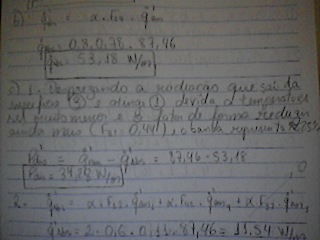
\includegraphics[scale=0.45]{./fig/5.png}
% \caption{\label{fig:3}3} 
% \end{center}
% \end{figure}

\myfig[scale=.28]{figPME2360-20111130-05}{}

Trocador de calor casco tubo

1 passe carcaça

2 passes no tubo

130 tubos de latão

\[\phi _{i} = 13.4mm\]
\[\phi _{e} = 15.9mm\]
\[2m/passe\]

- Escoamento Interno nos tubos

\[\bar{T}_{m}=\frac{20+40}{2}=30ºC\]

\[\rho = 997 kg/m^{3}\]
\[\mu = 855 \times 10^{-6}\]
\[c_{p} = 4179 J/kgK\]
\[Pr = 5.83\]
\[K = 613 \times 10^{-3}\]

\[Re = \frac{U \phi _{i}}{\nu} = \frac{U \phi _{i} \rho}{\mu}\]

\[Re = \frac{1.25 \times 0.0134 \times 997 } { 855 \times 10 ^{-6}} = 19531\]

Turbulento

L/D $>$ 10

\[\bar{Nu}_{D} = 0.023 Re_{D}^{4/5}Pr^{0.4}=126\]

\[\bar{h}=\frac{126 \times 613 \times 10^{-3}}{ 0.0134 } = 5767 W/m^{2}K\]

Coeficiente Global

\[\frac{1 A_{ext}}{U_{ext}A_{ext}}=\frac{A_{ext}}{h_{i}A_{i}}+\frac{A_{ext}\ln(D_{e}/D_{i})}{2 \pi KL}+\frac{A_{ext}}{h_{ext}A_{ext}}
\]

\[\frac{1}{U_{ext}}=\frac{A_{ext}}{h_{i}A_{i}}+\frac{A_{e}\ln(D_{e}/D_{i})}{2 \pi \times k_{latao} \times (130\times 2 \times 2)} + \frac{1}{h_{ext}}\]

Substituindo $U_{ext} = 3422 \ W/m^{2}K$  
\paragraph{Método da Efetividade}


\[NUT = \frac{UA}{C_{min}} = \frac{3422 \times \pi \times D_{e} \times 130 \times 2 \times 2}{4179 \times (\rho Veloc \pi \frac{Di^{2}}{4}) \times 130 } = 0.934\]



Em que 

\[\dot{m}_{agua} = 22.75 = (\rho Veloc \pi \frac{Di^{2}}{4}) \times 130\]

\[q_{max}= c_{min}(T_{h,e}-T_{c,e}) = 4179 \times 22.75 \times (325-293) = 3035 kW\]

Para $C_{r} = 0$, para todo o trocador de calor:

\[\varepsilon = 1 - \exp(-NUT)=1-\exp(-0.934)\] 

\[\varepsilon = 0.607\]
\[q = \varepsilon \times q_{max} = 0.607 \times 3035 = 1842 kW\]

\[\dot{q}=\dot{m}_{v}h_{lv}\]

\[\dot{m}_{v}=\frac{1842 \times 10^{3}}{2378 \times 10^{3}}\]

\section{11.70}

% \begin{figure}[h]
% \begin{center}
% 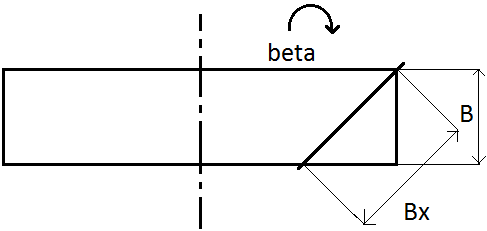
\includegraphics[scale=0.38]{./fig/4.png}
% \caption{\label{fig:4}4} 
% \end{center}
% \end{figure}

\myfig[scale=.28]{figPME2360-20111130-04}{}

\[T_{l,g}=1400K\]
\[cp_{g} = 11205 J/kgK\]
\[\dot{m}_{g}=10kg/s\]
\[\dot{m}_{agua}=3 kg/s\]
Entra x = 0(T=450K)

Sai x = 1 (T=450K)

\[U = 50 W/m^{2}K\]

Lembrando:

\[
\frac{1}{UA}=\frac{1}{U_{f}A_{f}}=\frac{1}{U_{q}A_{q}}=\frac{1}{(\eta_{0}hA)_{f}}+\frac{R_{i,f}^{''}}{(\eta_{0}A)_{f}}+ R_{p}+\frac{K_{i,q}^{''}}{(\eta _{0}A)_{q}} + \frac{1}{(\eta_{0}hA)_{q}}
\]

\[- NUT = \frac{UA}{c_{min}}\]

$c_{min}$, lado dos gases:
\[c_{min}=c_{p,g} \times \dot{m}_{g} = 1120 \times 10 = 11200 W/K\]

Mudança de fase, $c_{vapor} \rightarrow \infty$, $c_{r} \rightarrow 0$

Area de troca?

\[A = 500 \times \pi \times 0.025 \times L = 39.27 \ L\]
\[q_{max} = c_{min} \times (T_{h,e}-T_{c,e}) = 1200 \times (1400 - 450)\]
\[q_{max}= 10.64 \ MW\]
\[q_{trocador}=\dot{m}_{agua} \times h_{lv}\]
Em que $h_{lv}$ = $2024 \times 10^{3} \ J/kg$

\[\varepsilon = \frac{6.07}{10.64}=0.571\]

Trocador de calor com mudança de fase:

\[NUT = -\ln(1-\varepsilon)\]
\[NUT = -\ln(1-0.845)\]
\[NUT = \frac{UA}{c_{min}} = \frac{50 \times 39.27L}{ 11200 }\]
\[L = 4.82 m\]